%% Adaptado a partir de :
%%    abtex2-modelo-trabalho-academico.tex, v-1.9.2 laurocesar
%% para ser um modelo para os trabalhos no IFSP-SPO

\documentclass[
    % -- opções da classe memoir --
    12pt,               % tamanho da fonte
    openright,          % capítulos começam em pág ímpar (insere página vazia caso preciso)
    %twoside,            % para impressão em verso e anverso. Oposto a oneside
    oneside,
    a4paper,            % tamanho do papel. 
    % -- opções da classe abntex2 --schwinn
    % Opções que não devem ser utilizadas na versão final do documento
    %draft,              % para compilar mais rápido, remover na versão final
    paginasA3,  % indica que vai utilizar paginas em A3 
    BIBLATEX,           % indica para utilizar BIBLATEX em vez do abntex2cite
    REFINDENT,          % não fica exatamente no formato da ABNT, mas melhora muito a formatação
                        % não utilizar REFINDENT na versão final
    MODELO,             % indica que é um documento modelo então precisa dos geradores de texto
    TODO,               % indica que deve apresentar lista de pendencias 
    % -- opções do pacote babel --
    english,            % idioma adicional para hifenização
    brazil              % o último idioma é o principal do documento
    ]{ifsp-spo-inf-cemi} % ajustar de acordo com o modelo desejado para o curso
\AtBeginDocument

% ---
% Informações de dados para CAPA e FOLHA DE ROSTO
% ---
\titulo{DESENHO DO PROJETO}

% Trabalho individual
%\autor{AUTOR DO TRABALHO}

% Trabalho em Equipe
% ver também https://github.com/abntex/abntex2/wiki/FAQ#como-adicionar-mais-de-um-autor-ao-meu-projeto
\renewcommand{\imprimirautor}{
\begin{tabular}{lr}
Gabriel de Morais Ruiz & SP3046893 \\
Grazielli Lima Berti & SP3046966 \\
Gustavo Lourenço de Freitas & SP3049566 \\
João Vitor Silva Bispo & SP3052672 \\
Tayna Rita de França Souza & SP3050173 \\
Vinicius Almeida Soares & SP3046991 \\
Viviane de Santana Queiroz & SP3053601 \\
\end{tabular}
}


\disciplina{PI1A5 - Projeto Integrado I}

\preambulo{Entrega do desenho do projeto para a disciplina de Projeto Integrado I \LaTeX.}

\data{19/04/2022}

% Definir o que for necessário e comentar o que não for necessário
% Utilizar o Nome Completo, abntex tem orientador e coorientador
% então vão ser utilizados na definição de professor
\renewcommand{\orientadorname}{Professor:}
\orientador{JOSÉ BRAZ DE ARAUJO}
\renewcommand{\coorientadorname}{Professor:}
\coorientador{MARCELO TAVARES DE SANTANA}


% ---


% informações do PDF
\makeatletter
\hypersetup{
        %pagebackref=true,
        pdftitle={\@title}, 
        pdfauthor={\@author},
        pdfsubject={\imprimirpreambulo},
        pdfcreator={LaTeX with abnTeX2 using IFSP model},
        pdfkeywords={abnt}{latex}{abntex}{abntex2}{IFSP}{\ifspprefixo}{trabalho acadêmico}, 
        colorlinks=true,            % false: boxed links; true: colored links
        linkcolor=blue,             % color of internal links
        citecolor=blue,             % color of links to bibliography
        filecolor=magenta,              % color of file links
        urlcolor=blue,
        bookmarksdepth=4
}
\makeatother
% --- 

% carregando aqui referencias quando utilizando BIBLATEX
\IfPackageLoaded{biblatex}{%
\addbibresource{referencias.bib}
\addbibresource{exemplos/abntex2-doc-abnt-6023.bib}
}{}

% ----
% Início do documento
% ----
\begin{document}



% Retira espaço extra obsoleto entre as frases.
\frenchspacing 

%somente para o exemplo, fica primeiro

% -- lista de pendencias gerada pelo todonotes
% -- altere opções do usepackage para remover na versão final....

\newpage

% ----------------------------------------------------------
% ELEMENTOS PRÉ-TEXTUAIS
% ----------------------------------------------------------
\pretextual

% ---
% Capa
% ---
\imprimircapa

\newcounter{todocounter}
\newcommand{\todonum}[2][]
{\stepcounter{todocounter}\todo[#1]{\thetodocounter: #2}}

% ---

% ---
% Folha de rosto
% (o * indica que haverá a ficha bibliográfica)
% ---
\imprimirfolhaderosto
%\imprimirfolhaderosto*
% ---

% Quando registrado na biblioteca
%
% ---
% Inserir a ficha bibliografica
% ---

% Isto é um exemplo de Ficha Catalográfica, ou ``Dados internacionais de
% catalogação-na-publicação''. Você pode utilizar este modelo como referência. 
% Porém, provavelmente a biblioteca da sua universidade lhe fornecerá um PDF
% com a ficha catalográfica definitiva após a defesa do trabalho. Quando estiver
% com o documento, salve-o como PDF no diretório do seu projeto e substitua todo
% o conteúdo de implementação deste arquivo pelo comando abaixo:
%
% \begin{fichacatalografica}
%     \includepdf{fig_ficha_catalografica.pdf}
% \end{fichacatalografica}
\begin{fichacatalografica}
    \vspace*{\fill}                 % Posição vertical
    \hrule                          % Linha horizontal
    \begin{center}                  % Minipage Centralizado
    \begin{minipage}[c]{12.5cm}     % Largura
    
    \imprimirautor
    
    \hspace{0.5cm} \imprimirtitulo  / \imprimirautor. --
    \imprimirlocal, \imprimirdata-
    
    \hspace{0.5cm} \pageref{LastPage} p. : il. (algumas color.) ; 30 cm.\\
    
    \hspace{0.5cm} \imprimirorientadorRotulo~\imprimirorientador\\
    
    \hspace{0.5cm}
    \parbox[t]{\textwidth}{\imprimirtipotrabalho~--~\imprimirinstituicao,
    \imprimirdata.}\\
    
    \hspace{0.5cm}
        1. Palavra-chave1.
        2. Palavra-chave2.
        I. Orientador.
        II. Universidade xxx.
        III. Faculdade de xxx.
        IV. Título\\            
    
    \hspace{8.75cm} CDU 02:141:005.7\\
    
    \end{minipage}
    \end{center}
    \hrule
\end{fichacatalografica}
% ---



%Caso necessário
%% ---
% Inserir errata
% ---
\begin{errata}
Elemento opcional da \citeonline[4.2.1.2]{NBR14724:2011}. Exemplo:

\vspace{\onelineskip}


FERRIGNO, C. R. A. \textbf{Tratamento de neoplasias ósseas apendiculares com
reimplantação de enxerto ósseo autólogo autoclavado associado ao plasma
rico em plaquetas}: estudo crítico na cirurgia de preservação de membro em
cães. 2011. 128 f. Tese (Livre-Docência) - Faculdade de Medicina Veterinária e
Zootecnia, Universidade de São Paulo, São Paulo, 2011.

\begin{table}[htb]
\center
\footnotesize
\begin{tabular}{|p{1.4cm}|p{1cm}|p{3cm}|p{3cm}|}
  \hline
   \textbf{Folha} & \textbf{Linha}  & \textbf{Onde se lê}  & \textbf{Leia-se}  \\
    \hline
    1 & 10 & auto-conclavo & autoconclavo\\
   \hline
\end{tabular}
\end{table}

\end{errata}
% ---

%Obrigatório para trabalhos com bancas oficiais
%% ---
% Inserir folha de aprovação
% ---

% Isto é um exemplo de Folha de aprovação, elemento obrigatório da NBR
% 14724/2011 (seção 4.2.1.3). Você pode utilizar este modelo até a aprovação
% do trabalho. Após isso, substitua todo o conteúdo deste arquivo por uma
% imagem da página assinada pela banca com o comando abaixo:
%
% \includepdf{folhadeaprovacao_final.pdf}
%
\begin{folhadeaprovacao}

  \begin{center}
    {\ABNTEXchapterfont\large\imprimirautor}

    \vspace*{\fill}\vspace*{\fill}
    \begin{center}
      \ABNTEXchapterfont\bfseries\Large\imprimirtitulo
    \end{center}
    \vspace*{\fill}
    
    \hspace{.45\textwidth}
    \begin{minipage}{.5\textwidth}
        \imprimirpreambulo
    \end{minipage}%
    \vspace*{\fill}
   \end{center}
        
   Trabalho aprovado. \imprimirlocal, 24 de novembro de 2012:

   \assinatura{\textbf{\imprimirorientador} \\ Orientador} 
   \assinatura{\textbf{Professor} \\ Convidado 1}
   \assinatura{\textbf{Professor} \\ Convidado 2}
   %\assinatura{\textbf{Professor} \\ Convidado 3}
   %\assinatura{\textbf{Professor} \\ Convidado 4}
      
   \begin{center}
    \vspace*{0.5cm}
    {\large\imprimirlocal}
    \par
    {\large\imprimirdata}
    \vspace*{1cm}
  \end{center}
  
\end{folhadeaprovacao}
% ---


% ---- opcionais 

% -- resumo obrigatório
% ---
% RESUMOS
% ---

% resumo em português
\setlength{\absparsep}{18pt} % ajusta o espaçamento dos parágrafos do resumo
\begin{resumo}

Com o crescimento exponencial do uso da internet na última década, as redes sociais se mostraram o maior centro de socialização da sociedade moderna, local em que são pautadas uma infinidade de assuntos. Percebendo que, em meio a essa infinidade, existe a necessidade de evidenciação de algumas dessas pautas por vezes negligenciadas frente aos tópicos dominantes nas redes, surge o diversaGente. Esse é um aplicativo de rede social focado na melhoria de vida de pessoas com neurodiversidades e suas famílias a partir da criação de um ambiente em que elas sintam-se confortáveis para trocar experiências. E para tornar esse app possível, a metodologia ágil seguida para organizar e desenvolver do projeto baseia-se Scrum. Além disso, toda a documentação foi construída de acordo com as regras \ac{ABNT} e as tecnologias utilizadas no desenvolvimento integram o ecossistema JavaScript, as quais incluem React Native, Typescript, Node.JS, Nest.JS e Prisma.

 \textbf{Palavras-chaves}: rede social. neurodiversidades. projeto.

\end{resumo}

% resumo em inglês
\begin{resumo}[Abstract]
 \begin{otherlanguage*}{english}

With the exponential growth of internet usage in the last decade, social networks proved to be the biggest center of socialization of modern society, where it can be find a multitude of subjects. Realizing that in the midst of this infinity there is a necessity of highlighting some of these themes that are sometimes neglected in comparison to the mainstream topics on the social media, the diversaGente appears. It is a social network app focused on improving the lives of people with neurodiversities and their family by creating an environment where they feel comfortable to exchange experiences. And to build this app, the agile methodology followed to organize and develop the project is based on Scrum. In addition, the complete documentation complies with the \ac{ABNT} rules and the technologies used in development are part of the JavaScript ecosystem, which includes React Native, Typescript, Node.JS, Nest.JS and Prisma.

   \textbf{Keywords}: social networks. neurodiversities. project.
 \end{otherlanguage*}
\end{resumo}


% ---
% inserir lista de ilustrações
% ---
\pdfbookmark[0]{\listfigurename}{lof}
\listoffigures*
\cleardoublepage
% ---

% ---
% inserir lista de tabelas
% ---%
%\pdfbookmark[0]{\listtablename}{lot}
%\listoftables*
%\cleardoublepage
% ---

% ---
% inserir lista de quadros
% ---
\pdfbookmark[0]{\listofquadrosname}{loq}
\listofquadros*
\cleardoublepage
% ---


% ---
% inserir o sumario
% ---
\pdfbookmark[0]{\contentsname}{toc}
\tableofcontents*
\cleardoublepage
% ---


% ----------------------------------------------------------
% ELEMENTOS TEXTUAIS
% ----------------------------------------------------------
\textual


% ----------------------------------------------------------
% Introdução
% ----------------------------------------------------------
\chapter[Introdução]{Introdução}

Dispositivos móveis são amplamente utilizados pelos brasileiros, em 2019 82,7\% dos domicílios brasileiros possuíam acesso à Internet, e 98,6\% deles o faziam através de um telefone celular \cite{ibge2019}. Com este alto índice de uso surge também a grande popularidade das redes sociais no país e, por consequência da facilidade de disseminar informação, a necessidade de encontrar lugares confiáveis para se compartilhar e receber informações.

As redes sociais possibilitam a interação de milhões de pessoas, integrando grupos variados de diferentes lugares em um único ambiente virtual. Essas redes funcionam muito bem para lidar com as necessidades de interação da maioria das pessoas, mas não é possível afirmar que se encaixam perfeitamente para todos, afinal, existem públicos que requerem atenção diferenciada, um exemplo deles são as pessoas neurodiversas, que vivenciam uma rotina completamente destoante do convencional.

As barreiras e preconceitos que pessoas neurodiversas enfrentam na sociedade se iniciam já na dificuldade de acesso à informações corretas e confiáveis sobre o próprio termo que as englobam: neurodiversidade. Um termo designado à condição de pessoas cuja neurobiologia se desenvolveu de forma atípica em relação a um parâmetro médico e biológico que se designa como desenvolvimento normal na espécie humana. O T\ac{tdah} e o \ac{tea} são exemplos de diagnósticos comuns às pessoas neurodiversas e, apesar de todo o avanço científico dos últimos anos que possibilitam cada vez maior qualidade de vida, existem muitas barreiras de âmbito social que estas pessoas ainda enfrentam. Diante desse cenário, a socialização de milhares de pessoas neurodiversas é prejudicada e, muitas vezes, descredibilizada, e dado que o ser humano é um ser inerentemente social, o que ocorre é que elas têm uma necessidade elementar debilitada e por inúmeras vezes ignorada \cite{kanner43}.

Todo responsável por uma criança neurodiversa compreende a dificuldade existente desde o momento do diagnóstico, momento que traz uma enorme insegurança sobre como se dará o futuro da criança, até questões vistas como básicas do dia a dia. Atualmente, pouco se fala sobre as neurodiversidades, mas com pouca pesquisa pode-se descobrir que várias das pessoas que apresentam essas condições podem ter uma vida dita socialmente como normal, conseguindo brincar, estudar, trabalhar e construir relacionamentos sólidos, assim como outra pessoa não neurodiversa. O ponto de diferença é que, aquele que é diagnosticado com alguma divergência neurológica se desenvolve psicologicamente de forma específica, que varia de acordo com a neurodivergência em questão, e, muitas vezes, com alguma preocupação a mais em relação ao ambiente e estímulos externos (barulhos, toques e gestos, por exemplo). 

Pela existência das condições ditas é que o diversaGente se mostra um lugar cordial para pais, responsáveis e para as próprias pessoas neurodiversas, que não encontram com facilidade um ambiente em que tenham suas pautas evidenciadas e que possam encontrar pessoas com as mesmas questões e realidades.

\section{Objetivo}

A falta de acesso à informação a respeito de neurodiversidades como o Autismo, Síndrome de Rett, Distúrbio Abrangente do Desenvolvimento , Síndrome de Timothy, Síndrome de Angelman, Síndrome de Asperger e o Transtorno do Déficit de Atenção e Hiperatividade, por exemplo, é um problema que todo pai e mãe nessas condições enfrentam. O diversaGente tem como objetivo compartilhar conteúdos de qualidade com facilidade à informação para todos os pais e responsáveis de crianças neurodiversas. Como por exemplo notícias sobre neurodiversidade, boas escolas, médicos ao redor da sua localidade e aspectos de seus filhos divididos pelos pais em grandes fóruns de discussões. Não é uma rede social comum apenas para fazer amigos, é uma comunidade unida para troca de informação e conhecimento.


O aplicativo diversaGente tem como objetivo tornar-se um local disponível para que todos consigam compartilhar suas experiências, sejam elas dicas de vida a serem relatadas por meio do fórum ou experiências vividas em lugares específicos das quais queiram falar sobre e/ou fazer uma avaliação, trazendo pontos positivos do atendimento de um restaurante ou profissional de saúde, por exemplo.

Portanto, o diversaGente traz consigo a responsabilidade de transmitir maior volume e qualidade de informação acerca deste tema e, também, facilitar a comunicação entre esses pais, mães e responsáveis pelas crianças neurodiversas, criando, assim, uma comunidade unida em prol de uma causa e pronta para dar o apoio necessário àqueles que precisam.

\section{Justificativa}

Um estudo que reuniu dados da Hootsuite e WeAreSocial \cite{metropoles}, mostra que o Brasil é o terceiro no ranking de países que mais utilizam as redes sociais. De acordo com o estudo, os brasileiros ficam, em média 3h42 por dia conectados, ficando atrás somente das Filipinas (4h15) e Colômbia (3h45).
Já em relação às redes sociais, o Brasil conta com mais de 150 milhões de usuários, 70,3\% de sua população. O Sudeste aparece como a região com a maior taxa, cerca de 78\% dos usuários utilizam redes sociais.

Os dados em relação às neurodiversidades ainda não são muito divulgados, mas em relação ao autismo podemos destacar que uma em cada 44 crianças aos 8 anos de idade nos Estados Unidos é diagnosticada com o \ac{tea}, segundo relatório do \ac{cdc}, (publicado em 2.dez.2021). O número — com dados de 2018 — representa mais um aumento de 22\% em relação ao estudo anterior (1 para 54 — divulgado em 2020). Numa transposição dessa prevalência (de 2,3\% da população) para o Brasil, teríamos hoje, com uma estimativa baseado nos Estados Unidos, cerca de 4,84 milhões de autistas no país. Porém, ainda não temos números de prevalência de autismo no Brasil.

\begin{figure}[htb]
	
	\centering
	\caption{\label{fig_arq_virado}Prevalência de autismo nos \ac{eua} 2021}
	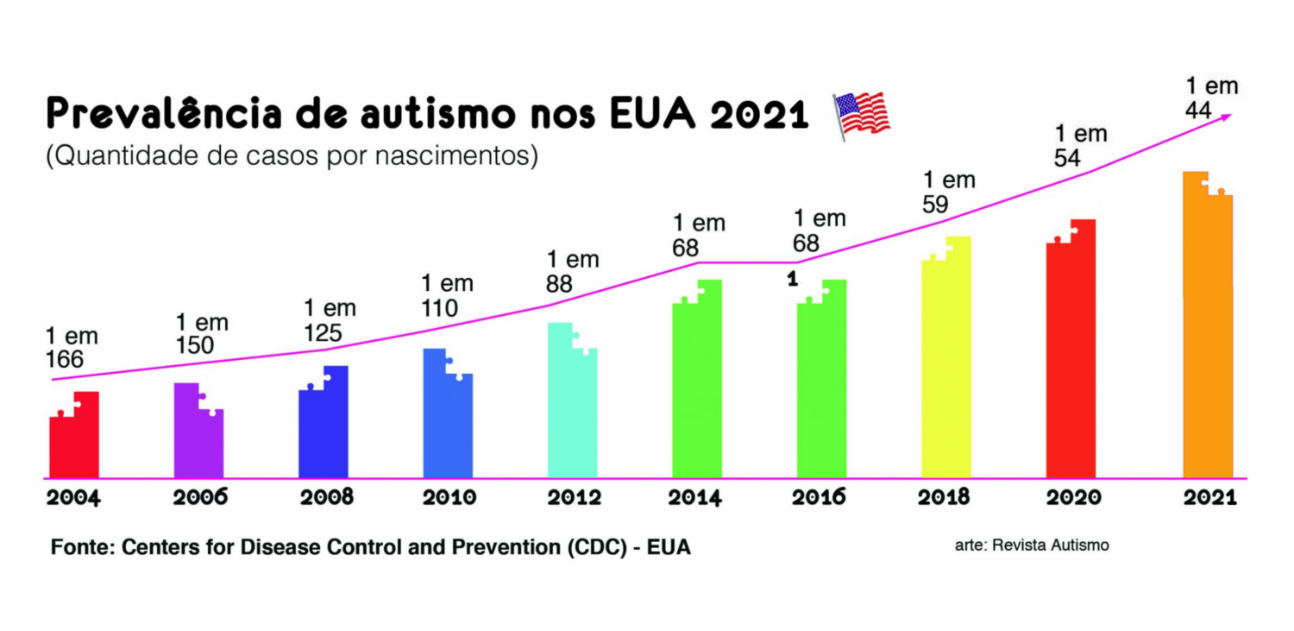
\includegraphics[width=0.9\textwidth]{anexos/diversaGenteGrafico.png}
\end{figure}

Tendo isso em mente, o diversaGente é um aplicativo destinado aos pais e mães de crianças Neurodiversas  pois é evidente que ter um filho com alguma neurodiversidade traz consigo vários desafios, como, por exemplo, encontrar escolas adequadas e um leque de profissionais especializados.

\section{Relato de usuário}

Conforme a concretização da ideia e o desenvolvimento do aplicativo avançaram, foi possível buscar um exemplo de aplicação real para um potencial usuário. Victoria Severiana, amiga do intregrante da equipe Gabriel Ruiz, é irmã de uma menina portadora da síndrome de Down e concordou em trazer um relato sobre a ideia e sobre o teste de uma versão beta do aplicativo.

"Em 2016, eu e meus pais soubemos que receberíamos uma criança com Síndrome de Down na família. Ainda na gestação, meus pais receberam a notícia e não souberam o que fazer com a informação, pois nunca tinham tido contato com nenhum portador ou parente. Inclusive, esconderam o fato por algumas semanas de mim (com 15 anos) e da minha outra irmã (com 10 anos), com medo de como lidaríamos com isso. Nesse momento, partindo do zero, eles se beneficiaram da facilidade da comunicação e da quantidade de informações encontradas na internet, buscando referências em fóruns, sites e grupos de redes sociais (GRAAC, APAE, Teleton, Grupo Pais de Crianças com Síndrome de Down do Facebook etc.). Depois do nascimento da minha irmã, Clara, também descobrimos que ela tinha uma doença cardíaca congênita, o que exigiu uma cirurgia de alto risco antes de 1 ano de idade. Outra condição que minha irmã também tem é a Paralisia de Bell. Todos esses fatos geraram ansiedade na família, que sempre buscou pelo melhor da Clara, e, sem dúvida, um app ou uma rede de apoio construída em torno de uma comunidade como o diversaGente teria facilitado muito os meios de chegar à informações úteis para o desenvolvimento dela. Hoje, já teríamos diversas recomendações para fazer dentro do app, sobretudo para círculos de crianças diversas na região Oeste de São Paulo: locais de terapia, a APAE de Cotia, estabelecimentos que são receptivos e adaptados a essas condições, tipos de alimentação, atividades lúdicas para desenvolvimento neural e motor etc., só para citar algumas coisas, pois conviver com uma criança diversa é aprender literalmente todos os dias."

Victoria Severiana da Silva, irmã da Clara, portadora da síndrome de Down.


E-mail para contato: victoriaseveriana@gmail.com


Telefone para contato: (11) 96329-1565


\section{Análise de concorrência}

A seção tem o intuito de, através de pesquisas na internet, traçar um comparativo de aplicativos com finalidades similares às do diversaGente e evidenciar as particularidades que esta tem em relação às outras. É possível ver no \autoref{tabela-comparativo} as características de cada aplicação para melhor visualização. 

O primeiro a ser comparado é o Facebook, além de ser uma das redes sociais mais usadas no Brasil e no mundo, possui algumas características similares com o diversaGente, como feed de postagem dentro de grupos, perfil pessoal e opção de compartilhamento de postagens. 

Para o Twitter, uma rede social que é um enorme fórum, muito utilizada entre os jovens, porém não possui nenhuma página para criar grupos e se conversar sobre um assunto específico. Possui um filtro bem eficiente que é possível buscar por algo, caso alguém já tenha feito uma postagem sobre. 

A Tismoo.me é a aplicação mais parecida com o diversaGente, possuindo também um fórum, nichada para o público de pais e responsáveis de crianças pertencentes ao espectro autista. O diversaGente consegue se diferenciar do Tismoo.me pelas funcionalidades de avaliação de locais, sendo possível compartilhar a experiência do usuário e também pela interação de chat em tempo real entre dois usuários. 

A característica principal da Emergency Chat é que pode ser utilizada em qualquer situação onde a fala é impossível, mas a comunicação ainda é necessária. Não é necessariamente uma rede social, possui um chat para comunicação.  

O TippyTalk é um aplicativo voltado para pais ou responsáveis de crianças neurodiversas, principalmente aquelas com alguma dificuldade de comunicação verbal. Permite que um administrador crie imagens exclusivamente identificáveis e familiares para as crianças, apoiando na educação e treino de atividades/tarefas rotineiras. 

O The Autism Helper também tem grande similaridade com o diversaGente porque é voltado para quem procura a facilitar, o máximo possível, a vida de indivíduos do espectro autista. O aplicativo possui fóruns para discussão e perfil pessoal. 



\
\begin{quadro}[thb]
	\centering
	\ABNTEXfontereduzida
	\caption[Comparativo entre aplicações]{Comparativo entre aplicações}	\label{tabela-comparativo}

	\begin{tabular}{|l|c|c|c|c|c|c|c|}
		\hline
		\thead{ } & \thead{diversa\\Gente} & \thead{Facebook}  & \thead{Twitter}  & \thead{Tismoo\\.me} & \thead{Emergency\\ Chat}  & \thead{Tippy\\ Talk}  & \thead{The \\Autism \\Helper}\\
		\hline
		Público Neurodiverso & X &  &  & X & X & X & X \\
		\hline
		Consultar Notícias & X &  & X & X &  &  &  \\
		\hline
		Fóruns & X & X &  & X &  &  & X \\
		\hline
		Locais Avaliados & X &  &  &  &  &  & \\
		\hline
		Chat & X & X & X &  & X & X &  \\
		\hline
		Feed de Postagem & X & X & X & X &  &  & X\\
		\hline
		Perfil Pessoal & X & X & X & X &  &  & \\
		\hline
		Buscar Usuários & X & X & X & X &  &  & \\
		\hline
		Compartilhar & X & X & X & X &  &  & X \\
		\hline
	\end{tabular}
\fonte{Equipe diversaGente (2022)}
\end{quadro}



% ---
% Capitulo de revisão de literatura
% ---
\chapter{Revisão da Literatura}

Neste tópico iremos fazer um estudo e tirar observações mais a fundo a respeito da neurodiversidade. Relatar quando começou os estudos a respeito das pessoas neurodiversas e
entender como foi o papel da sociedade no passado, no que nisso acarretou e as mudanças necessárias que surgiram para chegar nos dias de hoje.

\section{Influência do termo}
As questões neurodiversas em toda sociedade sempre foi um assunto difícil de falar, principalmente porque no passado era tratado com "modelo de tragédia pessoal" \cite{oliver1990politics}. Dessa maneira, foi crescendo o indiferente e inquestionável a respeito das pessoas que sofrem algum tipo de neurodiversidade. Entretanto, com os estudos, os teóricos que estudavam a causa mais fundo diziam que esse modelo social estaria equivocado, pois se deixar que essa percepção percorra nossa sociedade não irá trazer as necessárias responsabilidades sociais que devemos atingir para evitar esses equívocos. Sendo assim, essa mudança de responsabilidade para o comportamento com as neurodiversidades promove o empoderamentos do indivíduo e sendo assim ele ganha espaço para ser olhado pela sociedade e respeitado por elas.

\section{Virada de responsabilidades}
Um dos motivos que nos levou a trazer o tema da neurodiversidade para o projeto final está na maneira que o assunto é tratado na sociedade. Há muitos tabus a serem derrubados. Se, por volta de 1960, ainda se culpavam os pais pelos seus filhos terem nascido com alguma neurodiversidade e, portanto, impossibilitava o surgimentos de movimentos que pudessem entender e ajudar os familiares, hoje temos algumas conquistas a serem celebradas como projetos de leis que protejam as pessoas neurodiversas graças aos estudos sobre deficiência nos anos 70 que desconstruiu um modelo de responsabilidade única para uma socialmente construída.\cite{ortega2008}. Todavia, o preconceito, falta de informação e suporte ainda estão presentes no convívio social e dessa maneira, trazer uma rede social focada para sanar dúvidas e compartilhar informações e serviços torna-se esse assunto vivo diante a sociedade.

\section{Responsabilidade do Aplicativo}
Apontado no artigo de \cite{rios}, evidencia-se que no Brasil há um embate entre profissionais e pais a respeito do movimento neurodiverso, uma vez que a sociedade brasileira ainda está atrelada aos modelos ultrapassados lá da décadas de 1960. Dessa maneira, o diversaGente tem como objetivo tornar-se um ambiente de discussões e compartilhamento de informações sobre o assunto. Assim, o comprometimento na era digital que vivemos junto com a neurodiversidade nos remete ao compartilhamento de mais informações a respeito do assuntos com pessoas em diversos lugares, diversas famílias e culturas, pois em diversos artigos apresentam críticas a forma que os métodos atuais de tratamento são usados, uma vez que muitos tratamentos centram-se na deficiência e não na forma humana que deve ser tratado\cite{machado}. 


% ---


% Para facilitar a manutenção é sempre melhore criar um arquivo por capitulo, para exemplo isso não é necessário 
% Para facilitar a manutenção é sempre melhore criar um arquivo por capitulo, para exemplo isso não é necessário 

%---------------------------------------------------------------------------------------
\chapter{Escalabilidade}

O quesito ‘escalabilidade’ é muito abordado e de extrema importância atualmente, principalmente devido ao enorme fluxo de dados que corre dentre os sistemas e aplicações. A escalabilidade diz respeito a facilidade de crescimento da infraestrutura da aplicação de forma saudável, sem grandes impactos nos custos ferramentais e humanos e no desempenho da aplicação. Essa adaptabilidade pode estar relacionada com a implementação de novas funcionalidades, novas demandas de mercado, inserção em requisições legislativas e projetos de inovação, por exemplo. 

O projeto conta com ferramentas muito atuais, que já trazem consigo muito fortemente o conceito de escalabilidade, como o Heroku e o Docker, o primeiro que ganha cada vez mais espaço de mercado como uma Platform as a Service (PaaS), em que a solução permite que o desenvolvedor se desapegue de detalhes estruturais, trazendo maior facilidade de manutenção e maior agilidade de deploy, já o segundo possibilita a criação de ambientes virtuais completos, os chamados contêineres, que podem até mesmo ter seu crescimento automatizado de acordo com a demanda de requisições, gerando novos contêineres semelhantes, por exemplo. 

Por se tratar de um modelo de aplicação com pouca concorrência em mercado, existem chances relevantes de crescimento, assim, é possível que haja a necessidade de escalada da aplicação em um futuro breve, tendo isso em consideração, as ferramentas anteriormente citadas se encaixam muito bem nessa possível necessidade futura. 


%---------------------------------------------------------------------------------------
\chapter{Critérios de segurança}

\begin{itemize}
    \item A aplicação está de acordo com a Lei Geral de Proteção de Dados (LGPD, Lei nº13.709/2018). 
    
    \item Os dados que serão coletados e utilizados são: Como o usuário gostaria de ser chamado, foto do usuário opcional, data de nascimento, e-mail, neuroatipicidade da criança, localização aproximada opcional e senha. Não é obrigatório a publicação nem carregamento de dados pessoais que não queira disponibilizar ao público. 
    
    \item Para maior garantia de segurança, o armazenamento da senha será feito com criptografia e os dados dos usuários obterão total sigilo, sendo visíveis apenas pelo próprio usuário e por administradores do sistema em situações que sejam necessárias. 
    
    \item Os dados não sensíveis dos usuários (como nome de usuário e foto de perfil) serão visíveis para todos os usuários cadastrados, já dados sensíveis serão visualizáveis apenas pelo próprio usuário e, se necessário, pelos administradores da plataforma. 
    
    \item Os dados terão a sua integridade mantida, ou seja, não sofrerão alterações indevidas sem autorização do usuário, para que não possam vir a corromper a veracidade das informações. 
    
    \item Caso o usuário opte por encerrar sua conta, os seus dados pessoais não ficarão mais visíveis para outros usuários e seu perfil não deverá mais ser encontrado nas buscas dentro do aplicativo. Em 30 dias após o encerramento da conta todos os dados e informações da conta encerrada serão excluídos. 
\end{itemize}

%---------------------------------------------------------------------------------------
\chapter{Tecnologias a serem utilizadas}

Para o lado do cliente, iremos utilizar o React Native com Typescript junto a ferramenta Expo para testar o app com as APIs nativas do Android que essa ferramenta disponibiliza.

Já para o lado do servidor, utilizaremos Node.js com Typescript e framework NestJS para a construção da API, MongoDB como banco de dados, Prisma como ORM, Cloudinary como storage e para documentação de API, a especificação OpenAPI.

Para o ambiente de desenvolvimento, será utilizado o Docker a fim de obtermos facilidade em executar o projeto independente do Sistema Operacional local.

A hospedagem se dará por meio da Play Store para o app em React Native, do Heroku para o backend em Node.js e do MongoDB Atlas para o banco de dados.
Todo o versionamento será feito por meio das plataformas Github e Subversion.

Para realizar a prototipação das interfaces, será utilizada a ferramenta Figma e a construção de fluxos e brainstorms da equipe se darão por meio do Miro e Whimsical.

Por fim, para o gerenciamento do projeto, utilizaremos o Trello para registro de backlog e acompanhamento do status de desenvolvimento das histórias, o Discord para realização das cerimônias semanais da equipe e o WhatsApp para comunicações rápidas e mais urgentes entre o time.

\chapter{Manutenibilidade da aplicação desenvolvida}

\section{Ferramentas compatíveis com as tecnologias escolhidas para Testes automatizados e Análise Estática}
Usaremos Jest, um framework JavaScript para testes automatizados, e ESLint para análise estática do código.

\section{Sistemas de log para toda a aplicação}
Papertrail será o sistema de log que utilizaremos para mapear o comportamento da API em Node.js.

\section{Um processo de Integração Contínua}
A partir das Github Actions iremos estabelecer nosso workflow de CI (Continuous Integration).

\section{Especificação do “Coding Convention” (seja o próprio da linguagem, ou um criado/adaptado pela equipe)}
Usaremos o padrão recomendado pelo próprio ESLint para adequar:
\begin{itemize}
    \item Layout e formatação;
    \item Sugestão de alternativas para implementação do código (como, por exemplo, o uso do padrão camelCase para nomenclatura);
    \item Regras que visam corrigir possíveis problemas de lógica do código.
\end{itemize}
Todas as especificações a serem utilizadas estão disponíveis em: https://eslint.org/docs/rules/

\section{Design Patterns pertinentes à aplicação}
Utilizaremos os padrões Observer, Singleton e Injeção de Dependência.

\chapter{Diagrama de classes do sistema}
\begin{sidewaysfigure}[htb]

    \centering
	\caption{\label{fig_diag_virado}Diagrama de classes do sistema}
	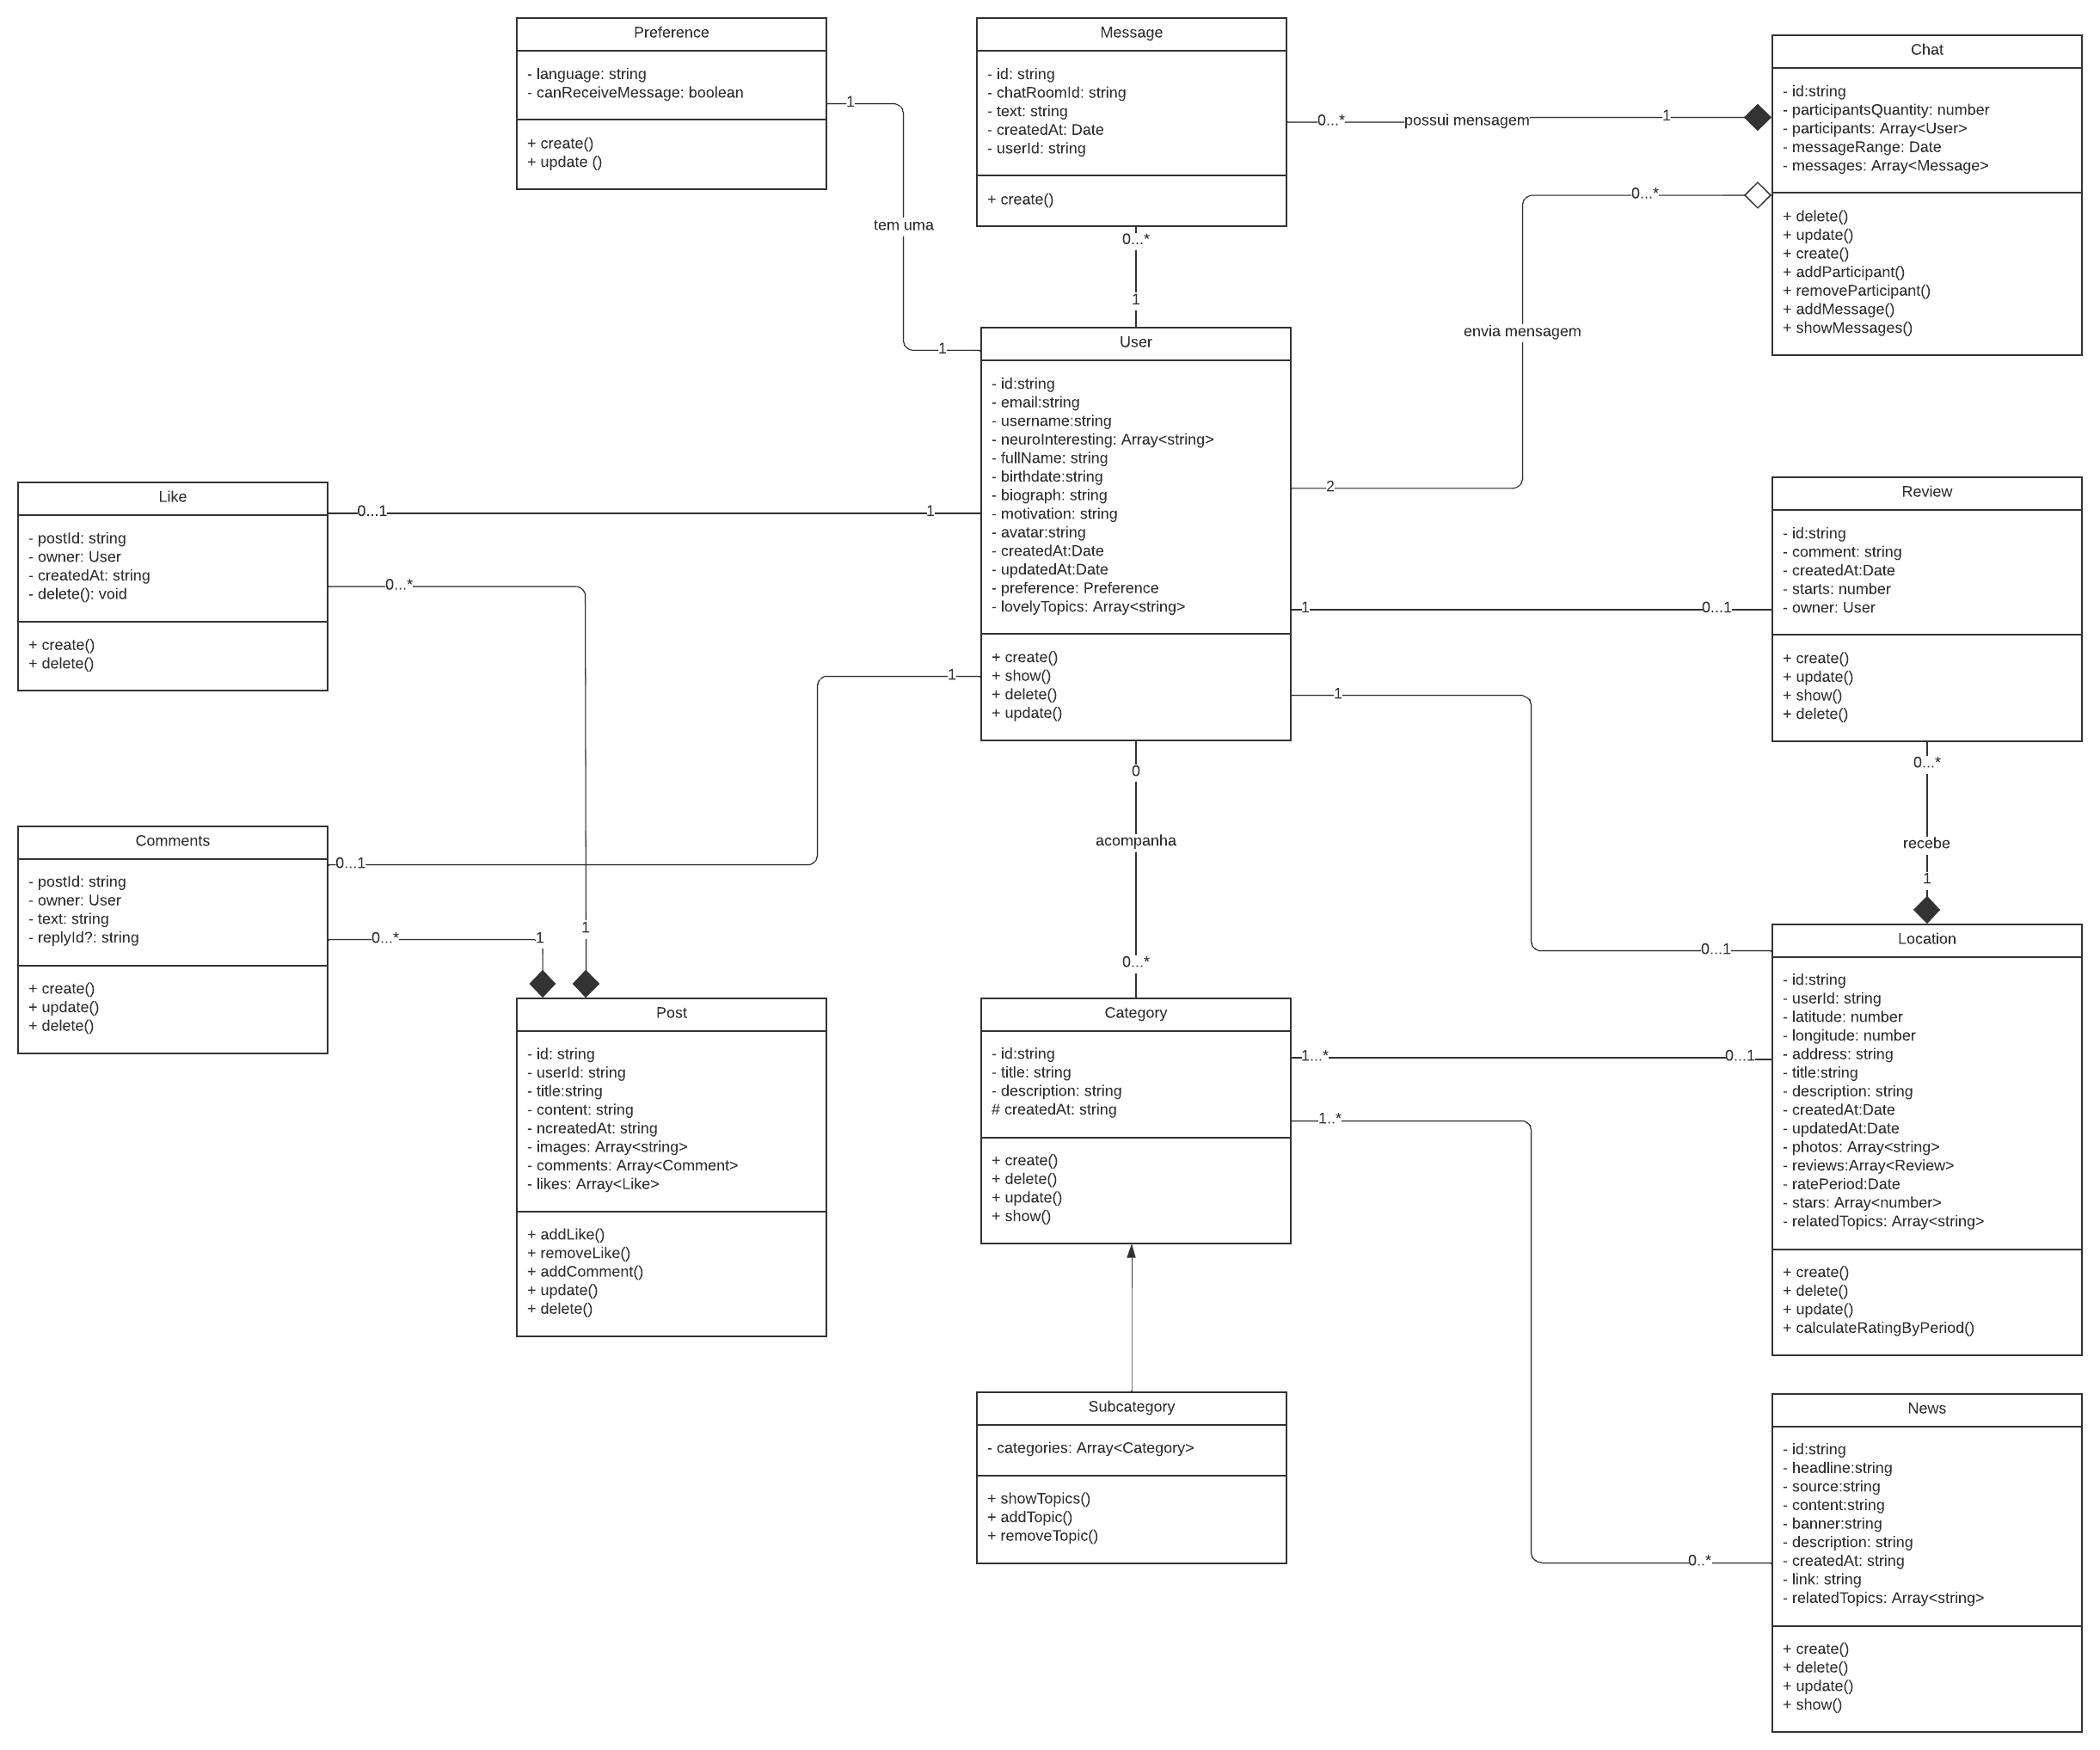
\includegraphics[width=0.9\textwidth]{anexos/diagrama.png}

	\end{sidewaysfigure}
%---------------------------------------------------------------------------------------







% exemplos de escrita LaTeX e erros comuns





% ---
% Conclusão (outro exemplo de capítulo sem numeração e presente no sumário)
% Dependendo do trabalho desenvolvido ele pode ter uma Conclusão ou Considerações finais
% Para trabalhos de disciplina utilizar Considerações Finais
% ---
\chapter{Considerações Finais}
% Exemplo de como adicionar linha adicional no sumário
Com a matéria de Projeto Integrado I e II (PI1A5 e PI2A6), foi possível vivenciar, de fato, as etapas e desafios que envolvem desenvolver um software e sua documentação.

A experiência de realizar o projeto envolveu, acima de tudo, dificuldades diversas às quais foram necessárias adaptações, fossem elas individuais ou da equipe inteira. Todas essas dificuldades foram de extremo valor, já que puderam mostrar o quão importante são alguns fatores como: comunicação, sinceridade, atenção e proatividade.

Como maiores pontos de dificuldade pelos quais a equipe passou, pode-se citar o conhecimento sobre o tema escolhido, conhecimento técnico sobre as ferramentas de desenvolvimento, gestão de tempo e informações sobre as requisições de cada entrega e, por fim, a documentação LaTeX. Para todos esses pontos de falha foi crucial que houvessem reuniões, alinhamentos e divisão de tarefas balanceadamente, para que não houvesse prejuízo para nenhuma das partes.

Foi preciso esforço de todos os membros da equipe para se informarem acerca do tema escolhido, a neurodiversidade, para que, dessa forma, fossem evitados equívocos de terminologias utilizadas e falta de fontes de informação sobre como é a rotina das pessoas neurodiversas. Quanto aos outros pontos de dificuldade pontuados, foram realizadas diversas agendas e conversas informais para disseminação de conhecimento entre os membros, para que, o quanto antes, todos estivessem alinhados sobre todos os pontos do projeto.

Ao fim do projeto foi possível perceber a evolução de todos os envolvidos, tanto em âmbitos técnicos quanto em quesitos comportamentais, além de ser possível perceber o quão mais entrosada a equipe estava.



% ----------------------------------------------------------
% Finaliza a parte no bookmark do PDF
% para que se inicie o bookmark na raiz
% e adiciona espaço de parte no Sumário
% ----------------------------------------------------------
\phantompart

% ----------------------------------------------------------
% ELEMENTOS PÓS-TEXTUAIS
% ----------------------------------------------------------

% ----------------------------------------------------------

% ----------------------------------------------------------
% Referências bibliográficas
% ----------------------------------------------------------
% quando não esta utilizando biblatex tem que carregar as referencias aqui
\IfPackageLoaded{biblatex}{%
\printbibliography

}{%
\bibliography{}
}

\bibliography{EQUIPE PM3. Product Owner: função, salário e tudo que você precisa saber sobre o papel [S.I] [2022]. Disponível <https://www.cursospm3.com.br/product-owner-o-que-faz-salario-habilidades/>. Acesso em: 09 de abr. 2022}
\\

\bibliography{REHKOPF, Max. Sprints [S.I] [2022?]. Disponível em <https://www.atla-\\ssian.com/br/agile/scrum/sprints> Acesso em: 09 de abr. 2022}
\\

\bibliography{REHKOPF, Max. O que é um scrum master? [S.I] [2018?]. Disponível em\\ <https://www.atlassian.com/br/agile/scrum/scrum-master>. Acesso em: 09 de abr. 2022}
\\

\bibliography{WEST, Dave. Planejamento do Sprint [S.I] [2022?]. Disponível em\\ <https://www.atlassian.com/br/agile/scrum/sprint-planning> Acesso em: 17 de abr. 2022}

\bibliography{Ortega, FranciscoDeficiência, autismo e neurodiversidade. Ciência & Saúde Coletiva [online]. 2009, v. 14, n. 1 [Acessado 30 Março 2022] , pp. 67-77. Disponível em: <https://doi.org/10.1590/S1413-81232009000100012>. Epub 20 Jan 2009. ISSN 1678-4561. https://doi.org/10.1590/S1413-81232009000100012.).}
\\

\bibliography{Moraes, Anna Victória Pandjarjian Mekhitarian, Bialer, Marina Martins e Lerner, RogérioCLÍNICA E PESQUISA DO AUTISMO: OLHAR ÉTICO PARA O SOFRIMENTO DA FAMÍLIA1 1 Apoio e financiamento: Fundação de Amparo a Pesquisa do Estado de São Paulo (FAPESP), pela concessão da bolsa de mestrado,número 18/03306-7 e do auxílio à pesquisa número 13/25332-6. . Psicologia em Estudo [online]. 2021, v. 26 [Acessado 18 Abril 2022] , e48763. Disponível em: <https://doi.org/10.4025/psicolestud.v26i0.48763>. Epub 10 Maio 2021. ISSN 1807-0329. https://doi.org/10.4025/psicolestud.v26i0.48763.}
\\

\bibliography{CARDIERI, Mariana Prates ESTUDOS CULTURAIS, NEURODIVERSIDADE E PSICANÁLISE: Um lugar para o autismo. UNIVERSIDADE FUMEC MESTRADO EM ESTUDOS CULTURAIS CONTEMPORÂNEOS. 2018, [Acessado 30 março 2022]. Disponível em: <https://repositorio.fumec.br/handle/123456789/139>. }
\\

\bibliography{Ana Carolina de Holanda Machado¹, Deborah Gerrane Damásio Nascimento¹, José Antônio da Silva Neto ¹, Mariana Ribeiro Rodrigues Alves¹, Vitória Daiany Guimarães Ramos¹, Júlia Maria Rodrigues de Oliveira². 1. Discente do curso de medicina do Centro Universitário de Anápolis - UniEVANGÉLICA. 2. Docente do curso de medicina do Centro Universitário de Anápolis - UniEVANGÉLICA. Revista Educação em saúde [RESU]. A relação entre a neurodiversidade e o Transtorno do Espectro Autista. [Acessado 30 março 2022]. Disponível em: < https://core.ac.uk/download/pdf/270182721.pdf >.}
\\

\bibliography{DIAS, Fabrízia Miranda de Alvarenga, DENUCCI, Moniki Aguiar, RODRIGUES, Daniele
Fernandes, SOUZA, Carlos Henrique Medeiros de. Transtorno do espectro autista e as concepções pragmáticas no contexto escolar. UENF, UFF, UENF, v. 27 n. 81 Supl. (2021) [Acessado 30 março 2022]. Disponível em: <https://www.revistaphilologus.org.br\\/index.php/rph/article/view/1056>. 
}
\\

\bibliography{RODRIGUES, F. A.; SANTANA, R. C. G. Contextualização de conceitos teóricos no processo de coleta de dados de redes sociais online. Informação & Tecnologia, v. 5, n. 1, p. 18-36, 2018. Disponível em: <http://hdl.handle.net/20.500.11959/brapci/110391>. Acesso em: 18 abr. 2022.}
\\

\bibliography{TOKARNIA, Mariana. Repórter da Agência Brasil - Rio de Janeiro. Celular é o principal meio de acesso à internet no país. Publicado em 29/04/2020. Disponível em: < https://agenciabrasil.ebc.com.br/economia/noticia/2020-04/celular-e-o-principal-meio-de-acesso-internet-no-pais>. Acesso em: 30 Março. 2022.}
\\

\bibliography{GABRIELA. Meu filho foi diagnosticado com autismo e agora?. Genial Care, 2020. Disponível em: (https://genialcare.com.br/blog/meu-filho-foi-diagnosticado-com-autismo-e-agora/). Acesso em: (30 março de 2022).}
\\
\bibliography{GISABELA. Neurodiversidade: a importância da inclusão. eCycle. Comportamento Disponível em: (https://www.ecycle.com.br/neurodiversidade/). Acesso em: (30 março de 2022).}
\\

\bibliography{MENDONÇA, Victor, ABREU, Tiago. Tudo o que você precisa saber sobre Neurodiversidade e Autismo. O Mundo Autista. Autismo. Disponível em: (https://omundoautista\\.uai.com.br/tudo-o-que-voce-precisa-saber-sobre-neurodiversidade-e-autismo/amp/). Acesso em: (30 março de 2022).}
\\

\bibliography{MENEZES, Clara. Redes sociais ajudam famílias a entenderem melhor o autismo. Portaldonic. Disponível em: (http://portaldonic.com.br/jornalismo/2017/07/17/redes-sociais-ajudam-familias-a-entenderem-melhor-o-autismo/). Acesso em: (30 março de 2022).}
\\

\bibliography{Francisco OrtegaI; Rafaela ZorzanelliI; Lilian Kozslowski MeierhofferII; Celita Almeida RosárioIII; Clarissa Freitas de AlmeidaIV; Bárbara Fonseca da Costa Caldeira de AndradaV; Beatriz da Silva ChagasV; Clara FeldmanV. IDepartamento de Políticas e Instituições de Saúde, IMS/UERJ. IIGraduanda, curso de Medicina, Universidade Federal do Rio de Janeiro. IIIAluna de Pós-graduação Lato Sensu em Saúde Pública, Escola Nacional de Saúde Pública Sérgio Arouca.
IVMestranda, Programa de Pós-graduação em Psicologia Social, UERJ.
VDoutorandas, Programa de Pós-graduação em Saúde Coletiva, IMS/UERJ. A construção do diagnóstico do autismo em uma rede social virtual brasileira. [Acessado 30 março 2022]. Disponível em: <https://www.scielosp.org/article/icse/2013.v17n44/119-132/#>.
}
\\

\bibliography{MENDONÇA, Sophia. Neurodivergentes: Autismo na Contemporaneidade. Manduruvá Edição Especiais, 2019. Link para o livro: https://www.google.com.br/books/edition\\/Neurodivergentes/xHAaEAAAQBAJ?hl=pt-BR&gbpv=0 }
\\

\bibliography{ABREU, Thiago. O que é neurodiversidade? Cânone Editoração Ltda, 2022. Link para o livro: https://www.google.com.br/books/edition/O_que_é_neurodiversidade\\/XCpcEAAAQBAJ?hl=pt-BR&gbpv=0}
\\

\bibliography{ Nicole Baumer, MD, MEd, Contributor, Julia Frueh, MD, Guest Contributor.  What is neurodiversity?. health.harvard. Disponível em: (https://www.health.harvard.edu/blog/what-is-neurodiversity-202111232645). Acesso em: (30 março de 2022).}
\\

\bibliography{exceptionalindividuals. Neurodiversity: Meanings, Types & Examples Find out more about the different types of neurodivergence. Disponível em: (https://exceptionalindividuals.com\\/neurodiversity/). Acesso em: (30 março de 2022).}
\\

\bibliography{SOUZA, Brenda, DESENVOLVIMENTO ATÍPICO E INCLUSÃO: CONCEPÇÕES DE ESTUDANTES DE CIÊNCIAS NATURAIS. Ciências Naturais [online]. 2001 [Acessado 30 Março 2022]: <https://bdm.unb.br/bitstream/10483/18192/1\\/2017_BrendaKevellynSouza_tcc.pdf>. }
\\

\bibliography{CANGUÇU, Raphael. O que são Requisitos Funcionais e Requisitos Não Funcionais? [S.I] [2021]. Disponível em <https://codificar.com.br/requisitos-funcionais-nao-funcionais/>. Acesso em: 15 de abr. 2022 }
\\

\bibliography{UNESP. Requisitos de Software [S.I] [2005]. Disponível em <https://www.dcce.ibilce.unesp.br/~ines/cursos/eng_soft/aula04.pdf>. Acesso em: 16 de abr. 2022}
\\

\bibliography{}
\\

\bibliography{}
\\

\bibliography{}
\\

\bibliography{}
\\

\bibliography{}
\\

\bibliography{}
\\

\bibliography{}
\\

\bibliography{}
\\

\bibliography{}
\\

\bibliography{}
\\

\bibliography{}
%---------------------------------------------------------------------
% INDICE REMISSIVO - Quando necessário 
% As palavras indexadas devem ser definidas com \index{} no texto
%---------------------------------------------------------------------
\phantompart
%---------------------------------------------------------------------

\end{document}